\documentclass[
  bibliography=totoc,     % Literatur im Inhaltsverzeichnis
  captions=tableheading,  % Tabellenüberschriften
  titlepage=firstiscover, % Titelseite ist Deckblatt
]{scrartcl}

% Paket float verbessern
\usepackage{scrhack}

% Warnung, falls nochmal kompiliert werden muss
\usepackage[aux]{rerunfilecheck}

% unverzichtbare Mathe-Befehle
\usepackage{amsmath}
% viele Mathe-Symbole
\usepackage{amssymb}
% Erweiterungen für amsmath
\usepackage{mathtools}

% Fonteinstellungen
\usepackage{fontspec}
% Latin Modern Fonts werden automatisch geladen
% Alternativ zum Beispiel:
%\setromanfont{Libertinus Serif}
%\setsansfont{Libertinus Sans}
%\setmonofont{Libertinus Mono}

% Wenn man andere Schriftarten gesetzt hat,
% sollte man das Seiten-Layout neu berechnen lassen
\recalctypearea{}

% deutsche Spracheinstellungen
\usepackage{polyglossia}
\setmainlanguage{german}


\usepackage[
  math-style=ISO,    % ┐
  bold-style=ISO,    % │
  sans-style=italic, % │ ISO-Standard folgen
  nabla=upright,     % │
  partial=upright,   % ┘
  warnings-off={           % ┐
    mathtools-colon,       % │ unnötige Warnungen ausschalten
    mathtools-overbracket, % │
  },                       % ┘
]{unicode-math}

% traditionelle Fonts für Mathematik
\setmathfont{Latin Modern Math}
% Alternativ zum Beispiel:
%\setmathfont{Libertinus Math}

\setmathfont{XITS Math}[range={scr, bfscr}]
\setmathfont{XITS Math}[range={cal, bfcal}, StylisticSet=1]

% Zahlen und Einheiten
\usepackage[
  locale=DE,                   % deutsche Einstellungen
  separate-uncertainty=true,   % immer Fehler mit \pm
  per-mode=symbol-or-fraction, % / in inline math, fraction in display math
]{siunitx}

% chemische Formeln
\usepackage[
  version=4,
  math-greek=default, % ┐ mit unicode-math zusammenarbeiten
  text-greek=default, % ┘
]{mhchem}

% richtige Anführungszeichen
\usepackage[autostyle]{csquotes}

% schöne Brüche im Text
\usepackage{xfrac}

% Standardplatzierung für Floats einstellen
\usepackage{float}
\floatplacement{figure}{htbp}
\floatplacement{table}{htbp}

% Floats innerhalb einer Section halten
\usepackage[
  section, % Floats innerhalb der Section halten
  below,   % unterhalb der Section aber auf der selben Seite ist ok
]{placeins}

% Seite drehen für breite Tabellen: landscape Umgebung
\usepackage{pdflscape}

% Captions schöner machen.
\usepackage[
  labelfont=bf,        % Tabelle x: Abbildung y: ist jetzt fett
  font=small,          % Schrift etwas kleiner als Dokument
  width=0.9\textwidth, % maximale Breite einer Caption schmaler
]{caption}
% subfigure, subtable, subref
\usepackage{subcaption}

% Grafiken können eingebunden werden
\usepackage{graphicx}
% größere Variation von Dateinamen möglich
\usepackage{grffile}

% schöne Tabellen
\usepackage{booktabs}

% Verbesserungen am Schriftbild
\usepackage{microtype}

% Literaturverzeichnis
\usepackage[
  backend=biber,
]{biblatex}
% Quellendatenbank
\addbibresource{lit.bib}
\addbibresource{programme.bib}

% Hyperlinks im Dokument
\usepackage[
  unicode,        % Unicode in PDF-Attributen erlauben
  pdfusetitle,    % Titel, Autoren und Datum als PDF-Attribute
  pdfcreator={},  % ┐ PDF-Attribute säubern
  pdfproducer={}, % ┘
]{hyperref}
% erweiterte Bookmarks im PDF
\usepackage{bookmark}

% Trennung von Wörtern mit Strichen
\usepackage[shortcuts]{extdash}

\author{%
Jan Philipp Jäkel\\%
\href{mailto:jan.jaekel@tu-dortmund.de}{jan.jaekel@tu-dortmund.de}%
\texorpdfstring{\and}{,}%
Piet Hoffmann\\%
\href{mailto:piet.hoffmann@tu-dortmund.de}{piet.hoffmann@tu-dortmund.de}%
}
\publishers{TU Dortmund – Fakultät Physik}


\subject{V601}
\title{Der Franck-Hertz-Versuch }

\date{
  \begin{align}
    \text{Durchführung: } & \text{24.5.2018} & \hspace{3em} & \text{Abgabe: 31.5.2018} \notag
%\\  \text{Korrektur: } & \text{} & \hspace {3em} & \notag
  \end{align}
}

\begin{document}

\maketitle
\thispagestyle{empty}
\tableofcontents
\newpage

\section{Theorie}
\label{sec:Theorie}
Ziel des Versuchs ist es die Quantennatur der Elektronenhülle eines Atoms nachzuweisen.
Mittels Elektronenstoßexperimenten ist es Beispielsweise möglich diese aufzuzeigen.
Stößt ein Elektron mit geeigneter Energie auf ein Atom, so wird das Atom aus dem Grundzustand auf seinen ersten angeregten Zustand gehoben.
Die Stoßpartner stoßen bei diesem Vorgang inelastisch.
Besitzt das Elektron die nicht den geeigneten Energiewert, dann stoßen Elektron und Atom elastisch und das Atom wird nicht angeregt.

\subsection{Der Frank-Hertz-Versuch}
Der Franck-Hertz-Versuch besteht aus einem evakuiertem Gefäß in dem sich Quecksilberdampf befindet.
Die Dampfdichte kann über die Umgebungstemperatur reguliert werden.
In das Gefäß ist ein Draht aus einem hochschmelzenden Metall eingeführt.
Wird dieser auf Rotglut erhitzt, so treten Elektronen aus, welchen den Draht wie eine Wolke umgeben.
Eine netzförmige Elektrode ist dem Draht gegenüber angebracht, an welcher eine positive Gleichspannung $U_B$ angelegt ist.
Durchlaufen die Elektronen die Strecke zwischen Glühdraht und Elektrode, so erhalten sie die kinetische Energie
\begin{equation}
  \label{eq:ekin}
  E_{kin} = e_0 U_B  ,
\end{equation}
wenn ihre Geschwindigkeit zu Beginn $v= 0$ beträgt.
Hinter der Beschleunigerelektrode befindet sich eine Auffängerelektrode.
Die Auffängerelektrode besitzt eine geringe Spannung gegenüber der der Beschleunigungsspannung.
Deshalb können nur Elektronen gegen das so entstehende Bremsfeld anlaufen, deren Geschwindigkeitskomponente in $z$-Richtung die Ungleichung
\begin{equation}
  \label{eq:ungl}
  \frac{m_0}{2}v_z^2 \geq e_0 U_A
\end{equation}
erfüllt.
Der Auffängerstrom $I_A$ kann mit einem geeignetem Messinstrument gemessen werden.
Im Beschleungigungraum befinden sich Hg-Atome.
Zwischen diesen und den Elektronen kommt es zu Zusammenstößen.
Ist die Energie der stoßenden Elektronen relativ gering, so treten elastische Stöße auf.
Aufgrund des großen Massenunterschieds der Stoßpartner ist die Energieübertragung des Elektrons an das Hg-Atom vernachlässigbar gering.
Im zentralen Stoß beträgt die übertragene Energie
\begin{equation}
  \label{eq:betrag}
  \symup\Delta E = \frac{4 m_0 M}{(m_0 + M)^2} E \approx \num{1.1e-5} E  .
\end{equation}
Die Richtungsänderungen, welche das Elektron erfährt können gravierend sein.
Erreicht die Elektronenenergie durch erhöhen von $U_B$ einen Wert der größer oder gleich der Energiedifferenz, zwischen dem ersten angeregten und dem Grundzustand des Hg-Atoms ist, so kann das Elektron das Hg-Atom anregen.
Das Elektron überträgt dabei genau den Energiebetrag $E_1 - E_0$ auf die Elektronenhülle des Hg-Atoms und behält den Restbetrag.
Das Hg-Atom befindet sich dann in dem ersten angeregtem Zustand.
Es geht mit einer Relaxationszeit in der Größenordnung $\SI{e-8}{\second}$ in den Grundzustand zurück, dabei emittiert es ein Photon mit der Energie
\begin{equation}
  \label{eq:phot}
  h\nu = E_1 -E_0    .
\end{equation}
Die Anregung des Hg-Atoms kann beobachtet werden indem der Auffängerstrom $I_A$ in Abhängigkeit der Beschleunigungsspannung $U_B$ gemessen wird.
Wird die Beschleunigungsspannung, ausgehend von Null, erhöht, dann Bewegen sich die von dem Glühdraht emittierten Elektronen weg von diesem.
Da eine anwachsende Zahl an Elektronen die Auffängerelektrode erreicht steigt der Auffängerstrom $I_A$ an.
Erreicht oder überschreitet die Energie der Elektronen den Wert $E_1-E_0$ ein wenig, sinkt der Auffängerstrom rapide ab.
Die Elektronen führen unelastische Stöße mit den Hg-Atomen durch, bei welchen sie fast ihre gesamte Energie übertragen.
Die Elektronen sind nicht mehr in der Lage gegen das Bremsfeld anzulaufen.
Wird die Energie weiter über die Beschleunigungsspannung gesteigert, so ist es ihnen wieder möglich Stöße mit den Hg-Atomen auszuführen.
Der Auffängerstrom steigt wieder an bis die Elektron erneut den Betrag $E_1-E_0$ erreicht haben.
Der Theoretische Verlauf des Auffängerstroms gegen die Beschleunigungsspannung ist in Abbildung \ref{fig:besch} dargestellt.
\begin{figure}[H]
  \centering
  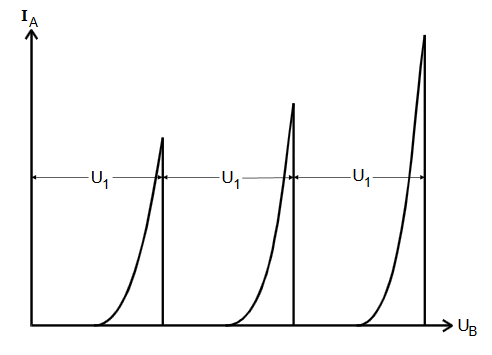
\includegraphics[width=0.8\textwidth]{content/theoriekurve.png}
  \caption{Idealisierter Zusammenhang zwischen Auffängerstrom und Beschleunigungsspannung\cite{v601}.}
  \label{fig:besch}
\end{figure}

\noindent Der Abstand zweier Maxima ist gleich dem ersten Anregungspotentials des Hg-Atoms:
\begin{equation}
  \label{eq:pot}
  U_1 = \frac{E_1 - E_0}{e_0}  .
\end{equation}
 \subsection{Einflüsse auf die Gestalt der Kurve}
Die tatsächlich gemessene Kurve weicht von der idealisierten Darstellung in Abbildung \ref{fig:besch} ab.
Dies geschieht aufgrund von verschiedenen Einflüssen.
\subsubsection{Einfluss des Kontaktpotentials}
In Glühdraht und Beschleunigerelektrode werden Materialien mit unterschiedlichen Austrittsarbeiten verwendet.
Damit eine hohe Elektronenemissionsrate erreicht wird, wird für den Glühdraht ein Material mit kleinerer Austrittsarbeit $\phi_G$ als die Austrittsarbeit $\phi_B$ der Beschleunigerelektrode verwendet.
Die Frank-Hertz-Kurve ist um den Wert
\begin{equation}
  \label{eq:k}
  K = \frac{\phi_B - \phi_G}{e_0}
\end{equation}
verschoben.
\subsubsection{Einfluss des Energie-Spektrums der Elektronen}
Die Elektronen treten bei Glühemission mit unterschiedlichen Geschwindigkeiten aus dem Glühdraht aus.
Es gibt keinen disktreten Energiewert für alle Elektronen, sondern eine statistische Energieverteilung.
Es gibt keine Unstetigkeiten in der Kurve.
Die Kurve fällt nicht wie in Abbildung \ref{fig:besch} nach einem Maximum mit negativ unendlicher Steigung auf Null, sondern nähert sich stetig einem Stromminimum.
\subsubsection{Einfluss des Dampfdrucks}
Notwendig für die Beobachtung der Franck-Hertz-Kurve ist ein bestimmter Stoßwahrscheinlichkeitsbereich zwischen Elektronen und Hg-Atomen.
Damit dies realisiert werden kann muss die mittlere freie Weglänge $\bar{w}$ klein gegen den Abstand zwischen Kathode und Beschleunigungselektrode sein.
Die Größe $\bar{w}$ kann über den Sättigungsdampfdruck $p_{sät}$ reguliert werden.
Es gilt:
\begin{equation}
  \label{eq:laeng}
  \bar{w}[\si{\centi\meter}] =\frac{\num{0.0029}}{p_{sät}}[\text{p in } \si{\milli\bar}]
\end{equation}
Der Sättigungsdampfdruck kann über die Innentemperatur geregelt werden.
Dieser kann über
\begin{equation}
  \label{eq:druck}
  p_{sät}(T) = \num{5.5e7} \exp\left(\frac{\num{-6876}}{T}\right)
\end{equation}
berechnet werden.
Wird der optimale Bereich stark unterschritten, dann wächst die Wahrscheinlichkeit, dass die Elektronen ohne Wechselwirkung von der Katode bis zu der Auffängerelektrode durchlaufen.
Wird der optimale Bereich stark überschritten, dann steigt zwar die Wahrscheinlichkeit, dass die Elektronen mit den Hg-Atomen wechselwirken,
es kommt aber auch zu elastischen Stößen, welche die Richtung der Elektronen ändern.
Die Zahl der Elektronen, welche die Auffängerelektrode erreichen, nimmt ab.

\section{Durchführung}
\label{sec:Durchführung}
Der Aufbau der Apparatur ist in Abbildung \ref{fig:aufbau} schematisch dargestellt.
\begin{figure}[H]
  \centering
  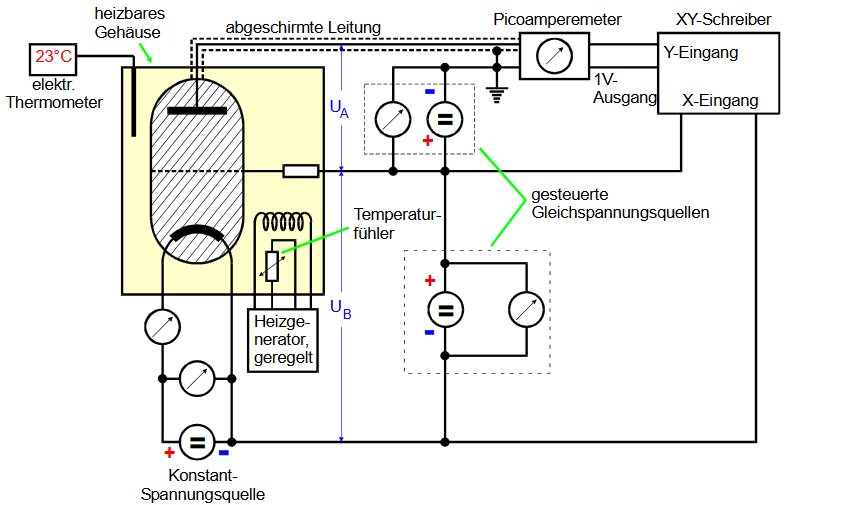
\includegraphics[width=\textwidth]{content/Aufbau.png}
  \caption{Aufbau des Versuchs\cite{v601}.}
  \label{fig:aufbau}
\end{figure}
\noindent Dieser besteht im Wesentlichen aus einem evakuiertem Gefäß.
In dem Gefäß befinden sich Hg-Dampf, Beschleunigerelektrode, Auffängerelektrode und Glühdraht.
Der Dampfdruck kann über einen Heizgenerator reguliert und die Innentemperatur über ein elektrisches Thermometer ausgelesen werden.
An die Auffängerelektrode ist ein Picoamperemeter angeschlossen.
An den Aufbau kann ein $XY$-Schreiber angeschlossen werden
\subsection{Energieverteilung der beschleunigten Elektronen}
\label{sec:ene}
Die Beschleunigerspannung wird auf konstante $U_B=\SI{+11}{\volt}$ eingestellt.
Die Temperatur wird auf ungefähr $\SI{20}{\degreeCelsius}$ gehalten.
Die Bremsspannung wird an den $X$-Eingang angeschlossen und die Auffängerstrom auf den $Y$-Eingang.
Die $X$-Achse des $XY$-Schreibers wird so geeicht, dass die Maximalspannung der Messung eine volle Auslenkung in $X$-Richtung erzielt.
Der Auffängerstrom $I_A$ wird in Abhängigkeit der Bremsspannung $U_A$ gemessen.
Dafür wird ein Diagramm mit dem $XY$-Schreiber erstellt.
Der Messung wird für eine Temperatur zwischen $T=\SI{140}{\degreeCelsius}$ %und $T=\SI{160}{\degreeCelsius}$
 wiederholt.
\subsection{Aufnahme von Franck-Hertz-Kurven}
Die Bremsspannung wird auf $U_A = \SI{1}{\volt}$ eingestellt.
Die Beschleunigerspannung wird an den $X$-Eingang angeschlossen und die Auffängerstrom auf den $Y$-Eingang.
Die Messung wird für einen Bereich von $0 < U_B < 60\si{\volt}$ durchgeführt.
Die $X$-Achse wird wie in Kapitel \ref{sec:ene} beschrieben geeicht.
Es werden Frank-Hertz-Kurven für die Temperaturen $T_1= 170\si{\degreeCelsius}$, $T_2= 180\si{\degreeCelsius}$ und $T_3= 190\si{\degreeCelsius}$ aufgezeichnet.
Die Kurve mit den am besten ersichtlichen Maximas wird ein weiteres mal in ein neues Diagramm eingezeichnet.
\subsection{Ionisierungsspannung von Hg-Atomen}
Die Temperatur wird innerhalb eines Bereichs von $T=100$ bis $110\si{\degreeCelsius}$ gehalten.
Die Bremsspannung wird auf einen festen Wert von $U_A = \SI{-30}{\volt}$ eingestellt.
Die Beschleunigerspannung wird an den $X$-Eingang und der Auffängerstrom an den $Y$-Eingang angeschlossen.
Die $X$-Achse wird wie in den vorhergehenden Messungen geeicht.
Die Messwerte werden von dem $XY$-Schreiber in einem Diagramm aufgetragen.

\section{Auswertung}
\label{sec:Auswertung}
\subsection{Bestimmung der Energieverteilung der Elektronen}
Die Messwerte zur Bestimmung der Energieverteilung bei $\SI{20}{\degreeCelsius}$ sind in Tabelle \ref{tab:e20} aufgetragen.
Die Messwerte werden dem Graphen des $XY$-Schreibers so entnommen, dass für große Steigung viele Werte aufgenommen werden.
Die Höhe ist hierbei eine Größe proportional zum Strom $I_A$.
\begin{table}[H]
    \caption{Messwerte der Energiekurve bei $\SI{20}{\degreeCelsius}$.}
    \label{tab:e20}
    \centering
    \begin{tabular}{S[table-format=2.3(0)e0] S[table-format=2.2(0)e0]}
        \toprule
{$U/\si{\volt}$} & { Höhe$/\si{\centi\meter}$} \\
		\midrule
1.000 &      14.65 \\
2.000 &      14.60 \\
3.000 &      14.50 \\
4.000 &      14.40 \\
5.000 &      14.20 \\
6.000 &      14.00 \\
6.500 &    13.85 \\
7.000 &      13.60 \\
7.500 &    13.30 \\
8.000 &      12.95 \\
8.500 &    12.40 \\
9.000 &      11.55 \\
9.250 &   10.95 \\
9.500 &    10.00 \\
9.625 &  8.70 \\
9.750 &   6.30 \\
9.813 &  4.5 \\
9.875 &  2.70 \\
10.000 &      1.00 \\
        \bottomrule
    \end{tabular}
\end{table}

\noindent Die differentielle Energieverteilung, welche sich ergibt aus $I_A(U_A)-I_A(U_A+\symup\Delta U_A)$ aufgetragen gegen $U_A$ aufgetragen, ist in Diagramm \ref{fig:e20} dargestellt.
\begin{figure}[H]
	\centering
	\includegraphics[width=0.8\textwidth]{build/energie20.pdf}
	\caption{Differentielle Energieverteilung der Elektronen bei $\SI{20}{\degreeCelsius}$.}
	\label{fig:e20}
\end{figure}

\noindent Aus dem Diagramm \ref{fig:e20} lässt sich nun über das Maximum das Kontaktpotential bestimmen:
\begin{equation}
	K = U_B - {U_B}_\text{eff} = \SI{1.19\pm0.06}{\volt}
\end{equation}
Wobei $U_B = \SI{11}{\volt}$ und ${U_B}_\text{eff} = \SI{9.813\pm0.063}{\volt}$, die Stelle des Maximums mit $\symup\Delta U_A$ als Unsicherheit.
\\
Die Messwerte für die Energieverteilung bei $\SI{140}{\degreeCelsius}$ sind in Tabelle \ref{tab:e140} aufgetragen.
Auch hier ist die Höhe proportional zu $I_A$.
\begin{table}[H]
    \caption{Messwerte der Energiekurve bei $\SI{140}{\degreeCelsius}$.}
    \label{tab:e140}
    \centering
    \begin{tabular}{S[table-format=2.1(0)e0] S[table-format=2.2(0)e0]}
        \toprule
{$U/\si{\volt}$} & { Höhe$/\si{\centi\meter}$} \\
		\midrule
0.0  & 14.60 \\
1.0  & 12.20 \\
2.0  & 9.45 \\
3.0  & 6.60 \\
4.0  & 3.85 \\
4.5  & 2.65 \\
5.0  & 1.90 \\
6.0  & 1.10 \\
7.0  & 1.30 \\
8.0  & 1.05 \\
9.0  & 0.60 \\
10.0 & 0.30 \\
       \bottomrule
    \end{tabular}
\end{table}

\noindent Die differentielle Energieverteilung ist in Diagramm \ref{fig:e140} zu sehen.

\begin{figure}[H]
	\centering
	\includegraphics[width=0.8\textwidth]{build/energie140.pdf}
	\caption{Messwerte der Energiekurve bei $\SI{140}{\degreeCelsius}$.}
	\label{fig:e140}
\end{figure}
\noindent

\subsection{Bestimmung der Anregungsenergie}
Um die Anregungsenergie des Qecksilbers zu bestimmen wird die Franck-Hertz-Kurve betrachtet, insbesondere der Abstand zwischen ihren lokalen Maxima, soweit diese noch erkennbar sind.
Die Abstände der Maxima sind in Tabelle \ref{tab:fh} aufgetragen.
\begin{table}[H]
    \caption{Messwerte der Energiekurve bei $\SI{140}{\degreeCelsius}$.}
    \label{tab:fh}
    \centering
    \begin{tabular}{S[table-format=1.2(0)e0]}
        \toprule
{$U_1/\si{\volt}$} \\
		\midrule
5.54 \\
4.57 \\
4.67 \\
4.78 \\
4.67 \\
4.89 \\
5.11 \\
       \bottomrule
    \end{tabular}
\end{table}

\noindent Für die Spannung $U_1$ ergibt sich ein Mittelwert von:
\begin{equation}
	\overline{U_1} = \SI{4.89\pm0.13}{\volt}
\end{equation}
Es ergibt sich somit eine Abstrahlungsfrequenz des Quecksilbers von
\begin{equation}
	\nu = \frac{e}{h}\, \overline{U_1} = \SI{1.18\pm0.3e15}{\hertz},
\end{equation}
wobei $h$\cite{plank} das Plank'sche Wirkungsquantum ist.

\subsection{Bestimmung der Ionisierungsenergie}
Zur Bestimmung der Ionisationsenergie wird aus dem zugehörigen Graphen der Bereich um die positiv steilste Stelle mittels linearer Regression gefittet.
Am Schnittpunkt der erhaltenen Gerade mit der $x$-Achse lässt sich $U_\text{ion} + K$ ablesen.
Die aus dem Graphen abgelesenen Messwerte sind in Tabelle \ref{tab:ion} aufgetragen.
Die Höhe ist wieder proportional zu $I_A$.
\begin{table}[H]
    \caption{Messwerte der Ionisationsenergie.}
    \label{tab:ion}
    \centering
    \begin{tabular}{S[table-format=2.2(0)e0] S[table-format=1.1(0)e0]}
        \toprule
{$U/\si{\volt}$} & { Höhe$/\si{\centi\meter}$} \\
		\midrule
25.00  & 2.1 \\
26.09  & 2.3 \\
27.17  & 2.6 \\
28.26  & 3.0 \\
29.35  & 3.3 \\
30.22  & 3.6 \\
       \bottomrule
    \end{tabular}
\end{table}
\noindent Der lineare Fit wird mit Python/SciPy mit der Vorschrift
\begin{equation}
	f(x) = mx+n
\end{equation}
erstellt und ist in Abbildung \ref{fig:ion} dargestellt.

\begin{figure}[H]
	\centering
	\includegraphics[width=0.8\textwidth]{build/ion.pdf}
	\caption{Messwerte und linearer Fit der Ionisationsenergiemessung.}
	\label{fig:ion}
\end{figure}
\noindent Die Parameter ergeben sich zu:
\begin{align}
	m &= \SI{0.29\pm0.01}{\centi\meter\per\volt} \\
	n &= \SI{-5.33\pm0.36}{\centi\meter}
\end{align}
Die Ionisationsspannung ergibt sich zu:
\begin{equation}
	U_\text{ion} = \frac{-n}{m} - K = \SI{17.19\pm1.40}{\volt} 
\end{equation}
Die Unsicherheit berechnet sich wie folgt:
\begin{equation}
	\symup\Delta U_\text{ion} = \sqrt{\left(\frac{\symup\Delta n}{m}\right)^2 + \left(\frac{n\symup\Delta m}{m^2}\right)^2 + \symup\Delta K ^2} 
\end{equation}

\section{Diskussion}
\label{sec:Diskussion}


\nocite{*}
\printbibliography{}

\end{document}
